\documentclass[11pt]{article}
\usepackage{amsmath}
\usepackage{graphicx}
\usepackage[margin=1in]{geometry}
\usepackage{float}


\title{
  CS 4993-049
  Final Report 
}
\author{
  Geethan Sundaram
}
\date{
  Dec 17, 2024
}

\begin{document}
\maketitle


\section{Introduction}

This report serves as documentation of the research conducted and the system built and configured for the Fall 2024 semester under the guidance and investigation of Prof Hyojoon (Joon) Kim and Ph.D. student Di Zhu.

This report will document my work throughout the semester, including the assembly and configuration of the system and my understanding of the simulation + emulation codebase of Lightning: MIT's Reconfigurable Photonic SmartNIC.

\section{Components}

These are the all relevant components that make up the system:

\begin{table}[H]
\centering
\renewcommand{\arraystretch}{1.5}
\setlength{\tabcolsep}{6pt} % Adjust cell padding
\begin{tabular}{|p{0.15\textwidth}|p{0.4\textwidth}|p{0.2\textwidth}|p{0.2\textwidth}|}
\hline
\textbf{Component} & \textbf{Description} & \textbf{Part} & \textbf{Manufacturer} \\ \hline
Optical Table & Holds the entire system. & T36H & Thorlabs \\ \hline
Laser Diode & Provides the laser/light source to be used for optical computations. & CLD1010LP, LPS-PM1550-FC & Thorlabs \\ \hline
Modulator & Modulates light amplitudes using input electrical voltages. & LNA2322 & Thorlabs \\ \hline
Photodetector & Converts modulated light to voltage; performs calculations in vector scenarios. & RXM15EF & Thorlabs \\ \hline
RF Amplifier & Amplifies voltage for ADC/DAC connections to photodetectors and modulators. & LMH5401EVM & Texas Instruments \\ \hline
Fiber Polarization Controller & Adjusts polarization state of light to stabilize fiber connections. & FPC031 & Thorlabs \\ \hline
FPGA (Field Programmable Gate Array) & Generates signals for deep learning inferences; integrates ADC/DAC for signal conversion. & EK-U1-ZCU111-G & AMD \\ \hline
\end{tabular}
\caption{Main Components}
\label{table:components}
\end{table}


\begin{table}[H]
\centering
\renewcommand{\arraystretch}{1.5}
\setlength{\tabcolsep}{6pt} % Adjust cell padding
\begin{tabular}{{|p{0.15\textwidth}|p{0.4\textwidth}|p{0.2\textwidth}|p{0.2\textwidth}|}}
\hline
\textbf{Component} & \textbf{Description} & \textbf{Part} & \textbf{Manufacturer} \\ \hline
Aluminum Clamp & Holds the photodetector, can be fixed onto to the SBE1 base via a screw. & ECM175 & Thorlabs \\ \hline
Base & Holds up the photodetector through connection to the ECM175 clamp above the optical table & SBE1 & Thorlabs \\ \hline
Clamping Fork & Fixes the SBE1 base to the table via a screw. & SCF1 & Thorlabs \\ \hline
\end{tabular}
\caption{Photodetector Supporting Parts}
\label{table:components}
\end{table}


\begin{table}[H]
\centering
\renewcommand{\arraystretch}{1.5}
\setlength{\tabcolsep}{6pt} % Adjust cell padding
\begin{tabular}{{|p{0.15\textwidth}|p{0.4\textwidth}|p{0.2\textwidth}|p{0.2\textwidth}|}}
\hline
\textbf{Component} & \textbf{Description} & \textbf{Part} & \textbf{Manufacturer} \\ \hline
Single Mode Patch Cable & Connects laser source to the first modulator. & P5-1550PMP-1 & Thorlabs \\ \hline
Polarization-Matching Patch Cable & Connects second modulator to the photodetector. & P5-SMF28Y-FC-1 & Thorlabs \\ \hline
Adapters & For connecting fibers between each pair of wires. & [Unknown] & Thorlabs \\ \hline
Modulator Supports & Keep the modulators embedded into the optical table. & 3D-Printed & MIT \\ \hline
\end{tabular}
\caption{Modulator Supporting Parts}
\label{table:components}
\end{table}


\begin{table}[H]
\centering
\renewcommand{\arraystretch}{1.5}
\setlength{\tabcolsep}{6pt} % Adjust cell padding
\begin{tabular}{{|p{0.15\textwidth}|p{0.4\textwidth}|p{0.2\textwidth}|p{0.2\textwidth}|}}
\hline
\textbf{Component} & \textbf{Description} & \textbf{Part} & \textbf{Manufacturer} \\ \hline
SMA Male-Male Cables & For all connections with RF amplifiers (from photodetector to ADC's, and DAC's to modulators). & ECM175 & Thorlabs \\ \hline
DC Power Supply & Provides a direct current (DC) to the RF amplifer. & SPS-3010 & Jesverty \\ \hline
Banana Plug to Alligator Clip Test Leads & Connects SPS-3010 DC power supply to RF amplifier. & E-LEADS-BTA-4 & SDTC Tech \\ \hline
1 Male to 2 Female Splitter & Splits voltage from DC Power Supply. & W21067 & WJSTN \\ \hline
\end{tabular}
\caption{RF Amplifier Supporting Parts}
\label{table:components}
\end{table}


\section{System Overview}

\subsection{Laser Diode}
The system begins with LP Pigtailed Laser Diodes (LPS-PM1550-FC) and a laser diode + temperature controller (CLD1010LP). The laser diode is responsible for converting the electricity it receives into light. This light is what is used for processing information and performing computation in photonic computing. 

The laser diode is mounted into the controller, allowing the functionality to control the intensity of the outputted light. This allows for the ability to control the amount of light that we may use for our computations, with greater amounts of light corresponding to greater capabilities for carrying information, processing power, and more.

The rest of the laser diode is a PM cable. An important distinction is understanding the difference between Single-Mode (SM) Fiber and Polarization-Maintaining (PM) Fiber cables. SM fiber transmits only one mode of light, or in other words only one path for the light to propogate through, where the light may be randomly polarized with waves that have different frequencies. PM cables, on the other hand, ensure that only one polarization of the inputted light, or a constant direction for the light's vector field, is propogated throughout the fiber. This leads to PM fiber having higher attenuation, or a reduction in the light's power.

\subsection{First Modulation}

Each modulator (LNA2322) contains a PM fiber cable to take in an inputted light and a SM fiber cable to output the resultant light. The PM fiber of the laser diode connects to an adapter that connects to the first modulator's PM input fiber. The purpose of the adapter is to connect the fibers between the two cables, allowing light to be transmitted between them.

The modulator receives its input voltage from the FPGA (EK-U1-ZCU111-G). This will be further explained in a later subsection.

The modulator takes in the input voltage and adjusts its amplitude, or its intensity. This is done by taking in the modulator's input voltage, and essentially multiplying it with the light's amplitude to produce an amplified light. It then outputs this through its SM fiber cable, which connects to an adapter that connects to another SM fiber cable. 

It should be known that the modulators do not come with supports, and there do not exist any supports for purchase for the modulators from the manufacturers. However, the supports are not complicated to design via computer-aided design (CAD). Additionally, Lightning provides $.stl$ files for modulator supports that are ready to be 3D printed.

\subsection{Fiber Polarization}

The SM fiber cable is inserted within a Fiber Polarization Controller (FPC031). The FPC allows for adjusting the polarization of the light within the SM fiber that is inserted within it, which will be obtained from the output of the first modulator. 

The FPC contains three paddles: a quarter-wave plate, a half-wave plate, and a quarter-wave plate in that order. The first quarter-wave plate is responsible for transforming the polarization state of the input light to be linear. The half-wave plate rotates the polarization state of the input. Finally, the second-quarter wave plate transforms the linear polarization stage back into an output arbitrary output state to travel through the fiber. 

The purpose of the FPC in the system is due to the output cable of the first modulator being SM fiber and the input cable of the second modulator being PM fiber. The FPC adjusts the polarization of the SM cable accordingly to ensure that when the light enters the PM cable, there is no change in polarization and the amplified light is correctly transmitted between the two modulators. To put it shortly, the FPC ensures consistency in terms of the light's polarization as it enters different types of fibers.

\subsection{Second Modulation}

Following the adjustment of the polarization, the SM fiber connects to an adapter that connects to the PM fiber cable that is attached to the the second modulator and responsible for inputting light.

The same process as the first modulator occurs, where the light is multiplied by the input voltage of the modulator. The resulting output light can actually be represented as photonic multiplication. 
\begin{itemize}
  \item In the first modulator, we are multiplying the amplitude by the first input voltage, a - $(a \times L)$
  \item In the second modulator, we are multiplying that product by the second input voltage, b - $(b \times (a \times L))$
\end{itemize}
  Due to associativity, in the end, we are essentially multiplying the light by the product of all the input voltages - $((b \times a) \times L)$.

  This double modulated light is then transmitted via SM fiber to the photodetector.

\subsection{Photodetector}

The photodetector (RXM15EF) takes in the double modulated light from the second modulator, and converts it into voltage.

The photodetector must be fixed to the table, which will require a base and clamping fork, which was the SBE1 base and the SCF1 fork. Optionally, we may include a post which would be attached over the base if we wish to elevate the photodetector a certain distance over the optical table. The photodetector comes with a clamp (ECM175), which would be attached to the post or base, depending on whether the post is used or not.

Due to the photonic multiplication of input voltages, the voltage produced by the photodetector is equivalent to the product of these input voltages.

\begin{figure}[H]
    \centering
    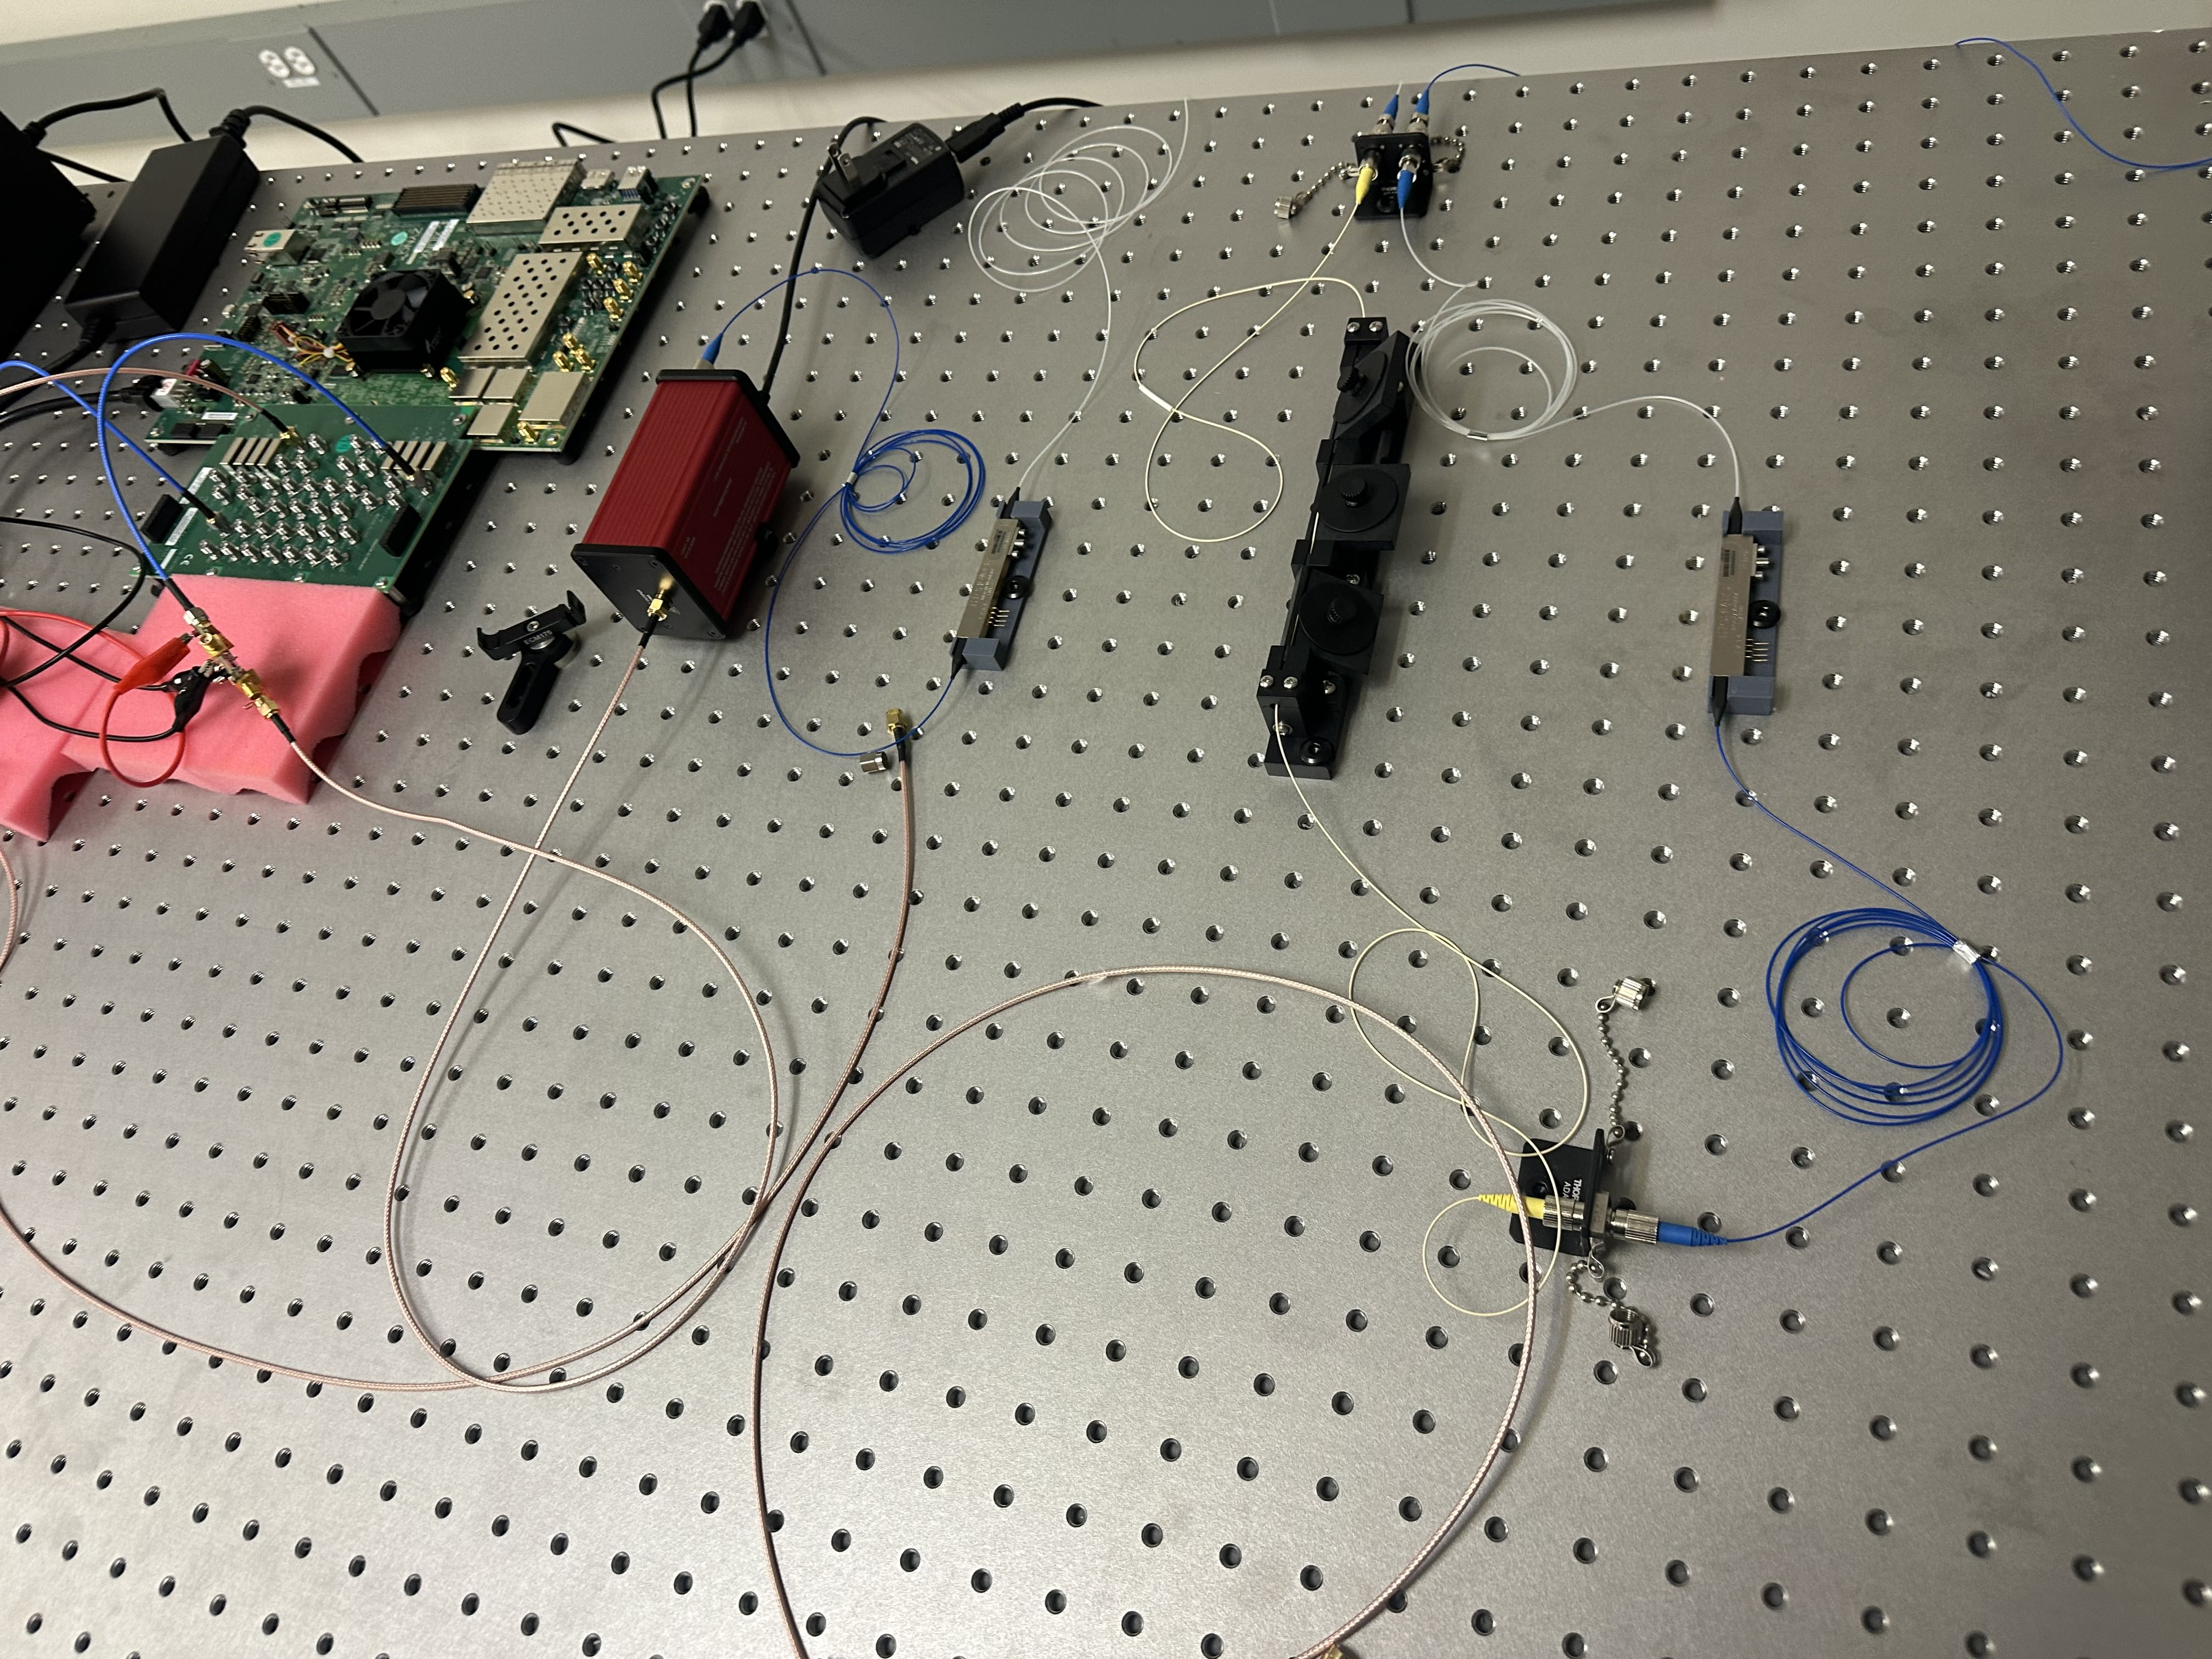
\includegraphics[width=0.5\linewidth]{modsandpd.jpg}
    \caption{Set up of Modulators, FPC, and Photodetector}
    \label{fig:enter-label}
\end{figure}

\subsection{FPGA}

The outputted voltage from the photodetector is sent to the FPGA (EK-U1-ZCU111-G). The FPGA is responsible for controlling the optical system and processing the computations that it performs. The FPGA supplies the datapath that allows  data to be efficiently processed and transmitted.

The FPGA sends the input voltages to the each of the modulators, supplying the proportion to multiply the light by in the optical domain. 

The FPGA has ADC's (analog-to-digital converters) and DAC's (digital-to-analog converters). The photodetector's voltage is send to an ADC, where it is converted into a digital input that the FPGA can read. Likewise, the FPGA sends signals to the DAC's to be converted into voltages that the modulators can take in.

\begin{figure}[H]
    \centering
    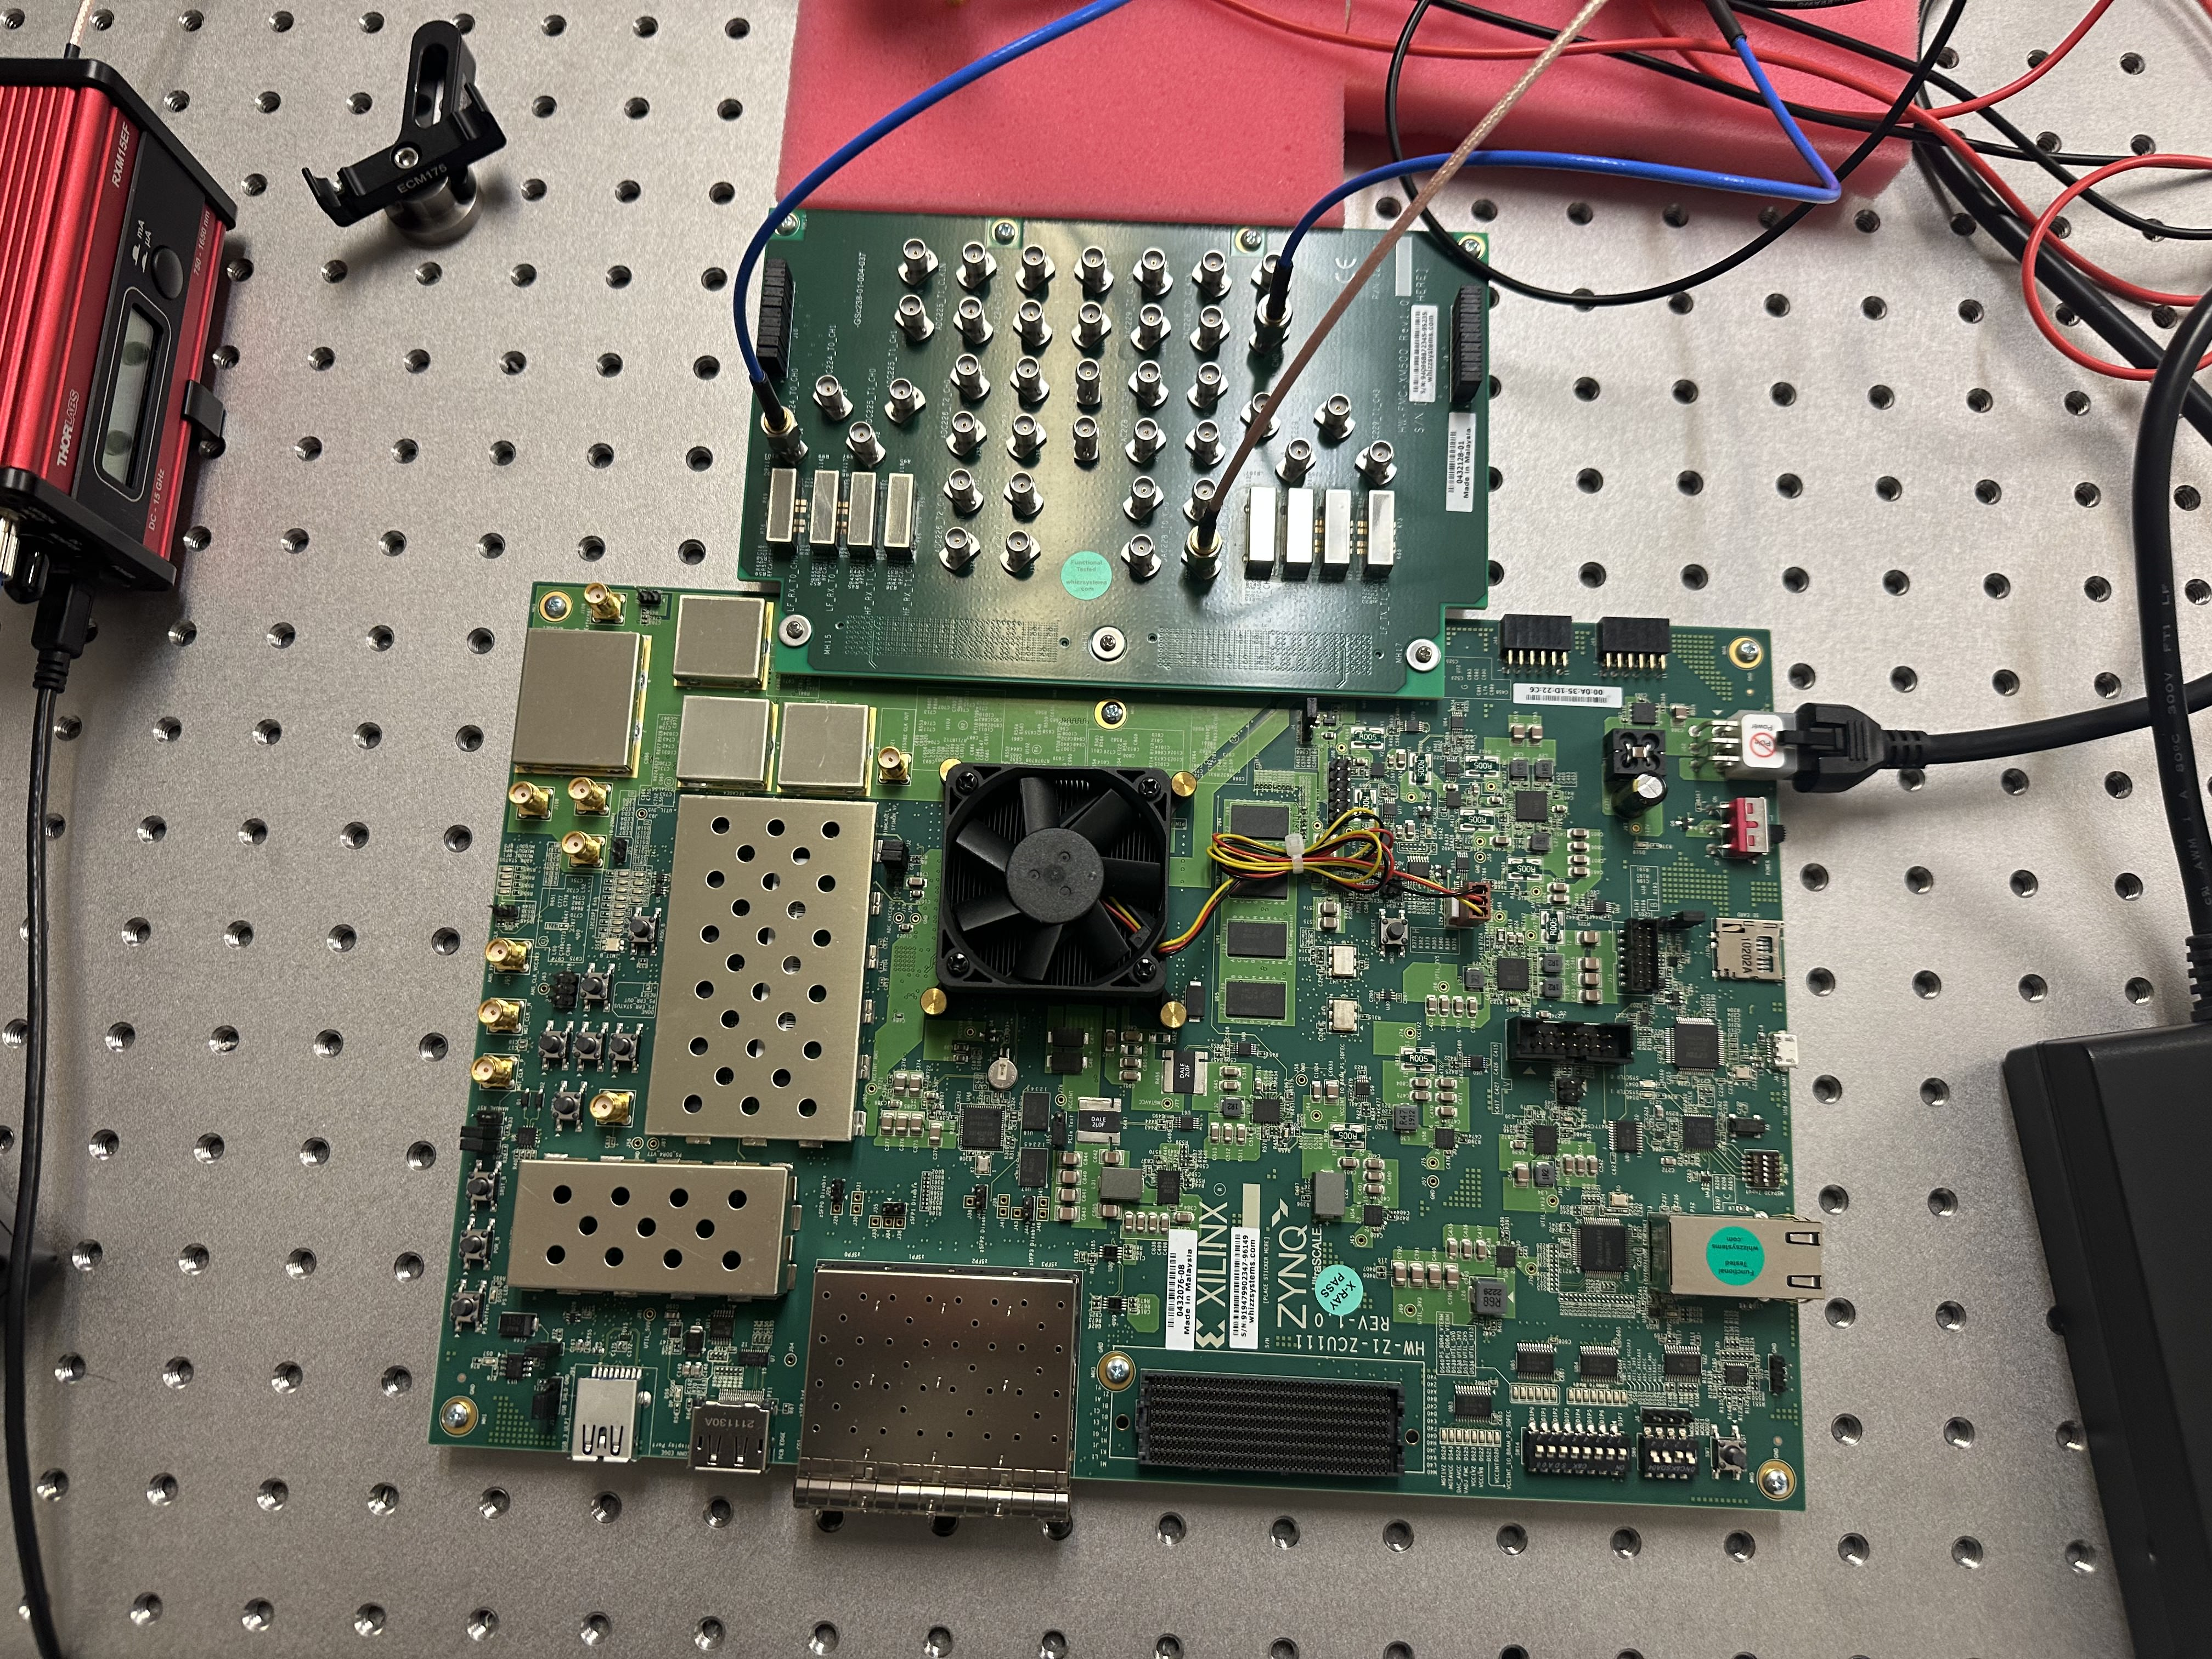
\includegraphics[width=0.5\linewidth]{fpga.jpg}
    \caption{FPGA with ADC's and DAC's}
    \label{fig:enter-label}
\end{figure}

\subsection{RF Amplifier}

The RF amplifiers (LMH5401EVM) are placed between the photodetector and the ADC and between each DAC and modulator. The outputted voltage from the DAC of the FPGA is insufficient for the modulator. To compensate for this lack of voltage, RF amplifiers amplify the voltage from the DAC before it reaches the modulator, ensuring a larger voltage range capable of matching the modulator's half-wave voltage. The photodetector's voltage is also insufficient for the ADC, requiring an additional RF amplifier to add additional voltage to the photodetector's output voltage to be sufficient (1.2 V CMV).

The RF amplifiers are powered by direct current (DC) and require DC power supplies to enable them to function.

\begin{figure}[H]
    \centering
    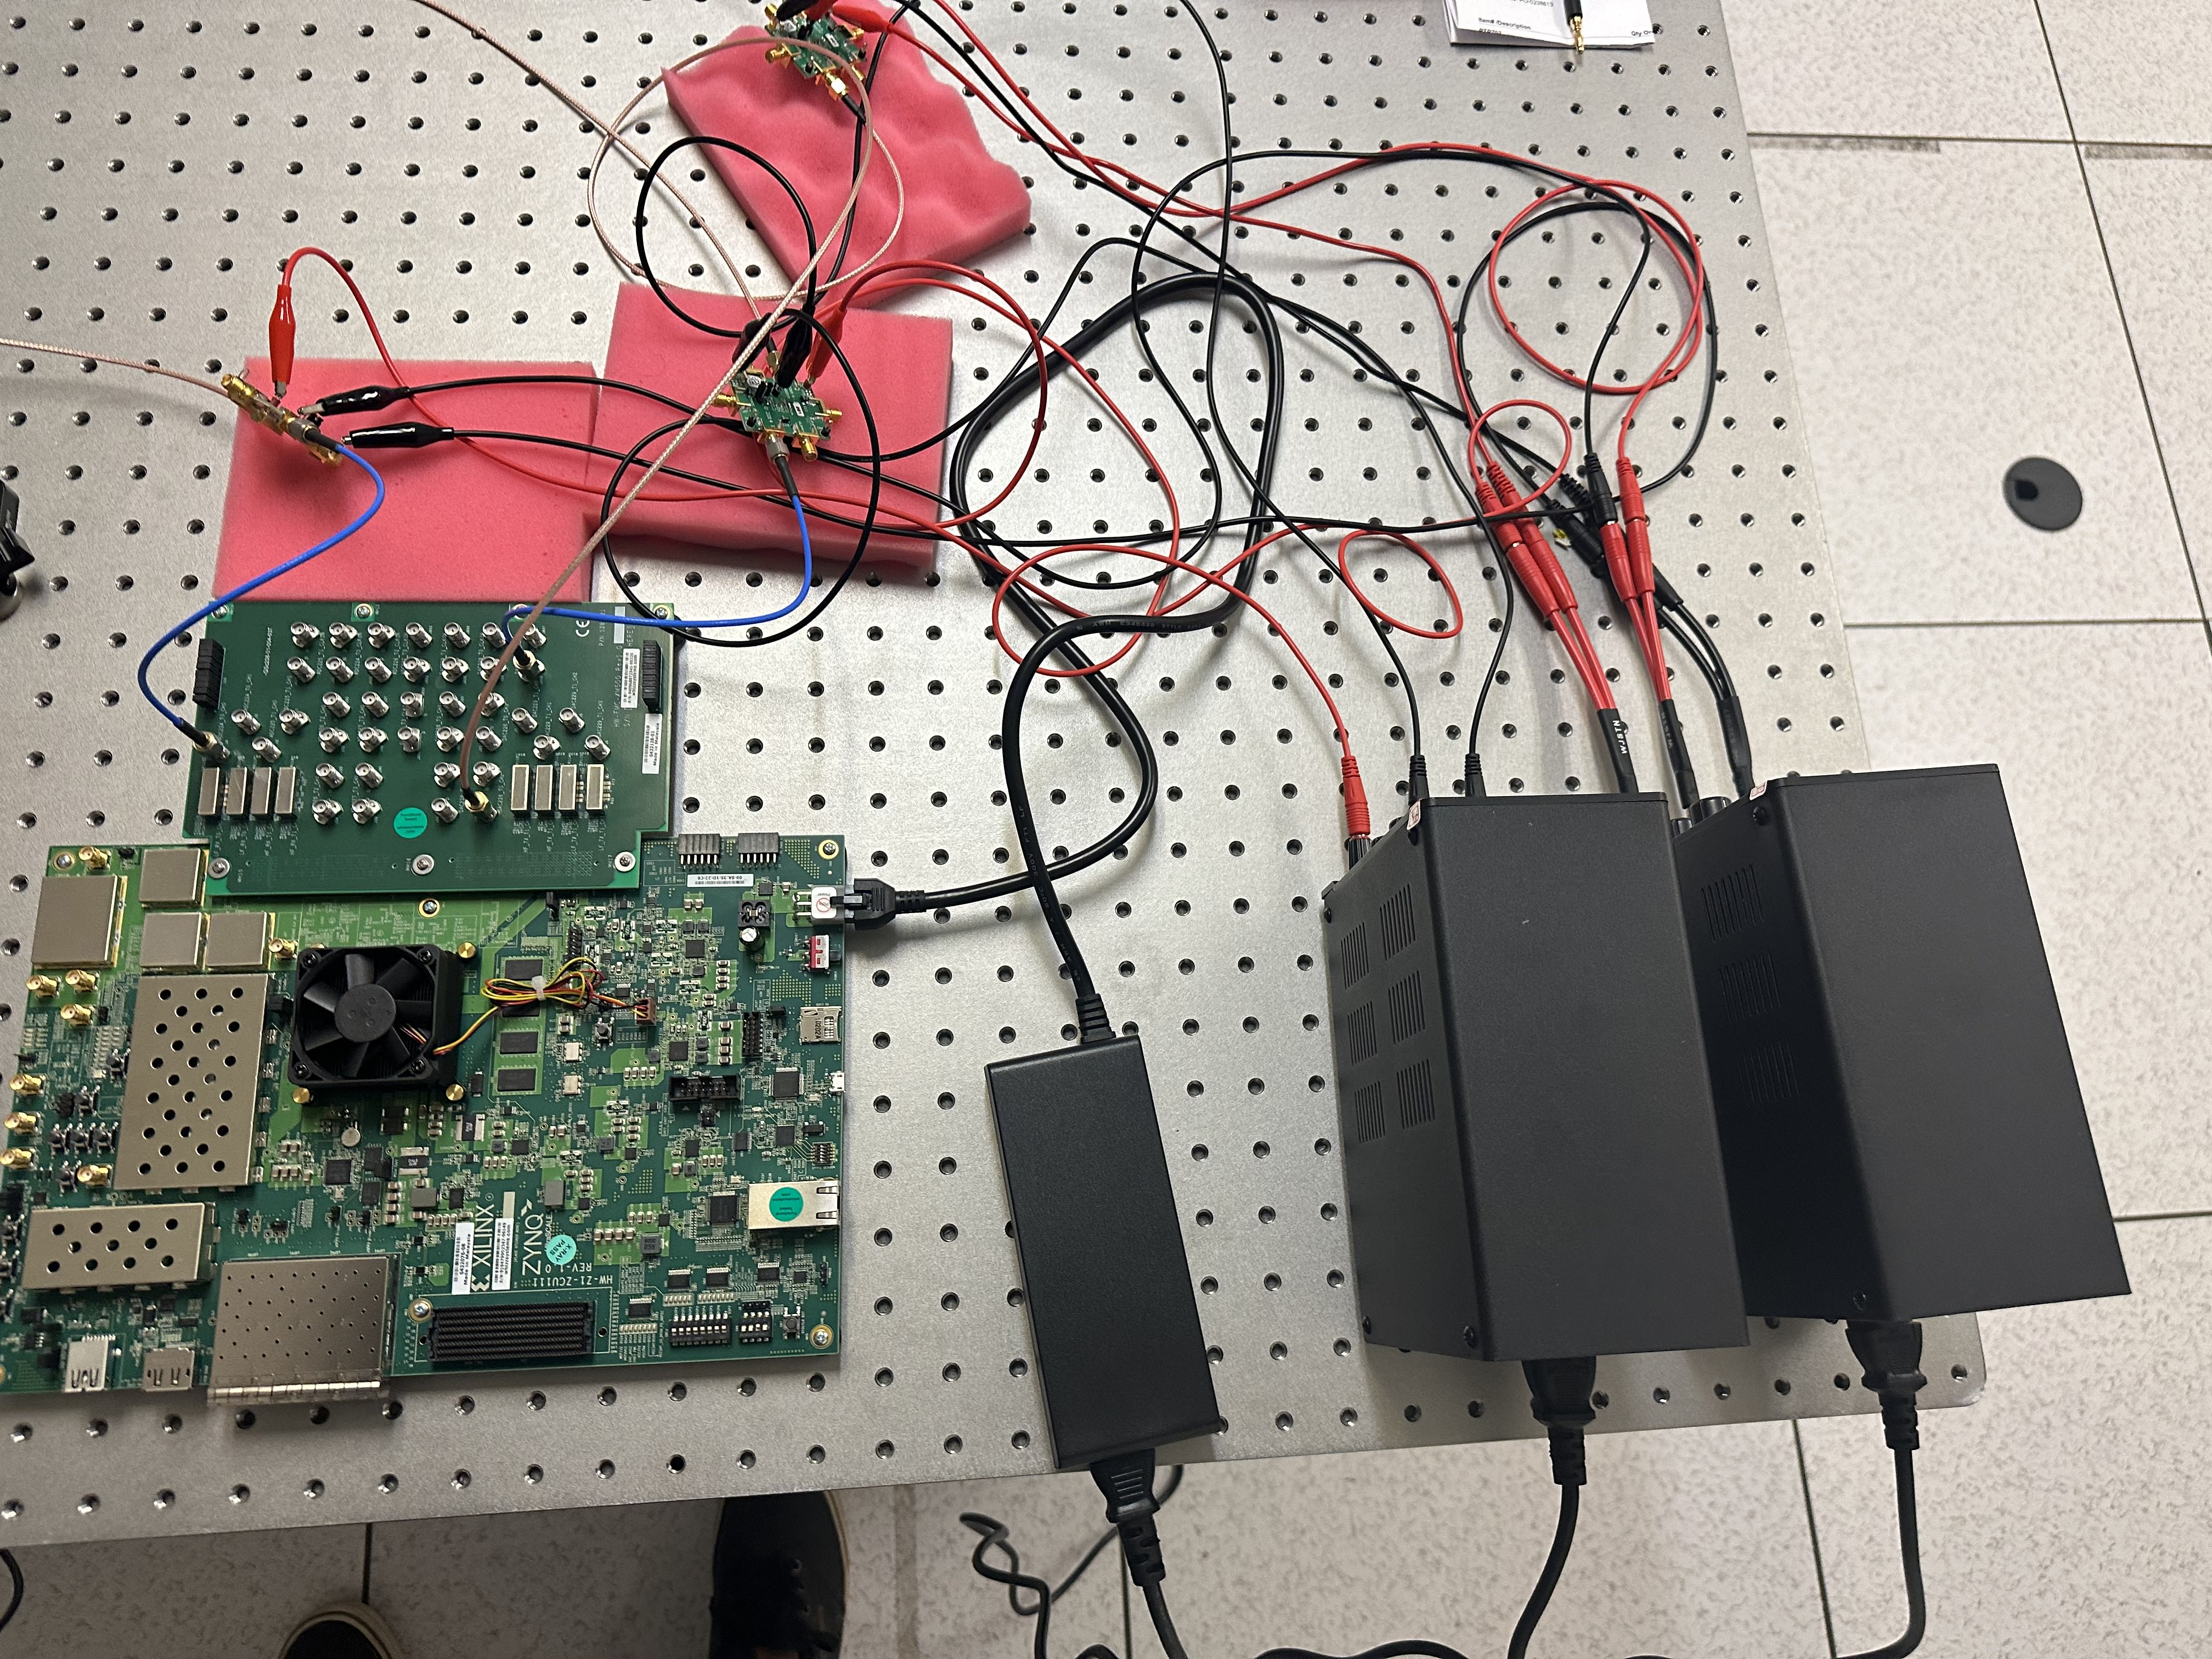
\includegraphics[width=0.5\linewidth]{rfamplifiers.jpg}
    \caption{RF Amplifiers with their power supplies}
    \label{fig:enter-label}
\end{figure}

\section{Lightning Simulation}

The purpose of the simulation is to see how Lightning compares to other processors in terms of speed and energy efficiency.

\subsection{Context}

The simulation aims to compare Lightning with an Nvidia A100 GPU, an A100X DPU, and a Brainwave smartNIC.

In the simulation, there are 10 pickle files with their own identification pickle number, each containing their own unique schedule of machine learning inferences for the simulator to go through.

In the simulation, a DNN inference is referred to as a request. A layer of the DNN inference is referred to as a job. 

\subsection{Process}
The process of the simulation is as follows:

\begin{enumerate}
    \item \textbf{bash run.sh} - Runs 4 simulations in parallel for each pickle file, each with one of the following processors: Lightning, Nvidia A100 GPU, A100X DPU, and Brainwave smartNIC.
    \begin{description}
        \item[sim.py] Runs a simulation
        \begin{enumerate}
            \item Parses command line arguments to get necessary parameters for processor, network speed, pickle number, final request, and more.
            \item Simulates the scheduling and processing of several DNN model requests on the inputted processor.
            \item Creates and configures a simulator instance to handle several requests with different arrive times and request rates based on network speed.
            \item The simulator processes all the requests and all the jobs within it.
            \item Calculates the average request time for each model after simulation is done.
            \item Retrieves and stores the count of the requests over time (how many requests were active during each point in time)
            
        \end{enumerate}
    \end{description}

    \item \textbf{bash csv\_gen.sh} - Converts the simulator's trial outputs to a readable CSV format
    \begin{description}
        \item[trial\_to\_csv.py] Converts trial log to CSV
        \begin{enumerate}
            \item Parses command line arguments to get necessary parameters for processor, network speed, pickle number, number of requests, and more.
            \item When average request completion time, total runtime, and count of active requests over time are all found, total runtime with average completion time per model and active requests over time are returned as strings
            \item If they are all not found, a string is stored with the partial data that is available
            \item The results are outputted into a CSV file using the strings
        \end{enumerate}
    \end{description}

    \item \textbf{bash final\_gen.sh} - Generates a TSV-formatted file containing the average runtimes of each DNN model with each processor
    \begin{description}
        \item[read\_csv.py] Processes runtime data for the DNNs on each processor and stores the results into a TSV-formatted file
        \begin{enumerate}
            \item Parses command line arguments to get necessary parameters for cores, batch size, and type of scheduling.
            \item For each pickle file, the corresponding CSV file is parsed
            \item For that pickle number, it finds ratios for other processors against Lightning for each model, tracking the maximum ratio
            \item Returns a string containing formatted runtimes and ratios
            \item The results are outputted into a TSV-format using the string 
        \end{enumerate}
    \end{description}

    \item \textbf{congestion\_plot.py} - Plots the active requests over time for each processor for the given network speed
    
    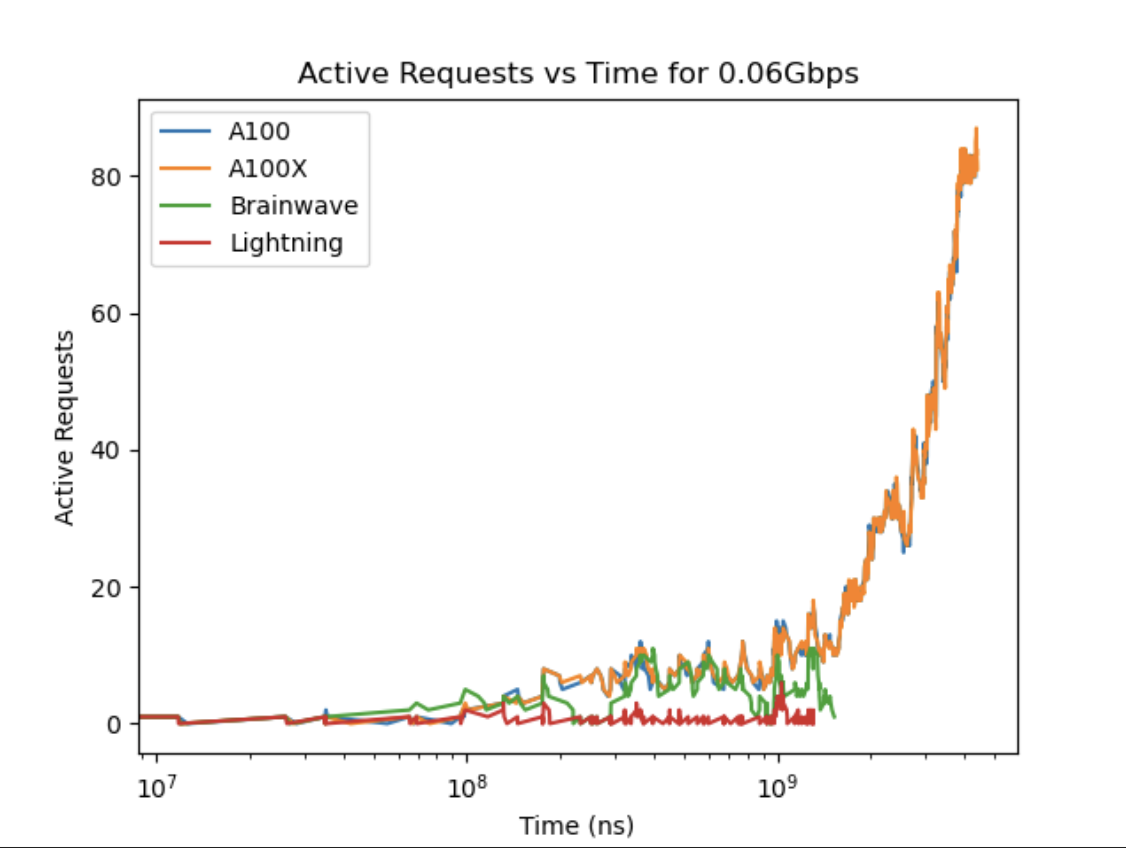
\includegraphics[scale=.75]{congestion.png}

    Note that Lightning remains the lowest curve, showing the least amount of requests marked during each noted point in time, indicating the least amount of request congestion overall.

\end{enumerate}

\section{Lightning Emulation}



\section{Conclusion}

\end{document}